\chapter{A calibrated finite-record response test}
\label{completion:statistics}

An exact response difference becomes an experiment only after preparation,
control, detection and sampling have been specified. This chapter turns the
preceding classical response constraint into a conservative finite-record test.
The conclusion is rejection of a declared classical model class. It is not a
device-independent certification of quantum behavior.

\section{Three settings and one predeclared direction}
Use independent fresh preparations in three settings: an unperturbed baseline,
a selective pulse held through readout at time $t_1$, and the same pulse held
through readout at time $t_2$. Each record is a binary detector outcome.
Let $p_0,p_1,p_2$ denote nominal outcome probabilities. The protected classical
contract implies
\begin{equation}\label{completion:samesign}
 (p_1-p_0)(p_2-p_0)\geq0.
\end{equation}
This follows for a singleton endpoint or a validated entrance-gateway region,
with native stationary preparation and a constant selective channel change.
The two pulse times are fixed in advance. The condition also survives
independent positive timing jitter when the same control remains applied.
A useful robustness is that the two arms need not have exactly the same
retention factor. Each may have its own constant $0\leq r_s<1$, provided it
suppresses the same native channel and leaves the other dynamics unchanged.
Each endpoint population displacement is a positive multiple of the same
signed quantity $-J_e$.
Exact retention calibration is needed for quantitative power and current
estimation, rather than for this qualitative same-sign consequence.
A delay after releasing the control requires a new calculation.

A common binary detector with false-positive rate $d_0$ and gain $k$ maps
population $p$ to $d_0+kp$. It preserves~\eqref{completion:samesign}, even if
$k<0$; $k=0$ removes the contrast. The known lower contrast used for power
must include this gain. A fixed shared offset cancels from both contrasts.
Setting-dependent offsets, preparation errors, control cross-talk and
unmodeled readout delays do not automatically cancel.

Let actual fixed Bernoulli probabilities $\widetilde p_s$ obey
$|\widetilde p_s-p_s|\leq\eta_s$, $s=0,1,2$. These are independently
justified complete-setting envelopes. Take $n$ independent records per arm,
also independent across arms, and form empirical frequencies $\widehat p_s$.
Predeclare the alternative orientation $p_1<p_0<p_2$. Write
\[
 \widehat d_1=\widehat p_0-\widehat p_1,
 \qquad\widehat d_2=\widehat p_2-\widehat p_0.
\]
Reject the protected classical contract only when both
\begin{equation}\label{completion:reject}
 \widehat d_1>\eta_0+\eta_1+h_\alpha,
 \qquad
 \widehat d_2>\eta_0+\eta_2+h_\alpha.
\end{equation}
Otherwise report an inconclusive result. Do not switch the orientation after
examining the data without a corresponding multiple-testing adjustment.

\begin{theorem}[False rejection and power]
Suppose the stated preparation, intervention, detector, independence and
calibration contract holds. If
\[
 n h_\alpha^2\geq\log(1/\alpha),
\]
the test~\eqref{completion:reject} has false-rejection probability at most
$\alpha$ uniformly over the protected classical class.
If a specified alternative has certified nominal gaps
$p_0-p_1\geq g_1>0$, $p_2-p_0\geq g_2>0$, and
\[
 h_\alpha+h_\beta\leq
 m:=\min\{g_1-2(\eta_0+\eta_1),\ g_2-2(\eta_0+\eta_2)\},
 \qquad n h_\beta^2\geq\log(2/\beta),
\]
then its probability of rejection is at least $1-\beta$.
\end{theorem}
\begin{proof}
A difference of independent empirical Bernoulli frequencies, each based on
$n$ records, is a sum of $2n$ bounded terms with squared range sum $2/n$.
Hoeffding's inequality therefore gives each one-sided deviation bound
$\exp(-nh^2)$. Under~\eqref{completion:samesign}, at least one of the two
nominal directed contrasts is nonpositive. Its actual mean is at most its
two calibration radii. Rejecting both inequalities implies an upper-tail
deviation of this particular contrast, hence the bound $\alpha$. This is an
intersection--union test; sharing the baseline creates no extra union factor
for false rejection.

Under the alternative, the actual mean of contrast $i$ is at least its
nominal gap minus its two calibration radii. Its rejection threshold contains
the same radii once more. Thus failing that threshold requires a downward
deviation of at least $h_\beta$. A union bound over the two possible failures
gives $2\exp(-nh_\beta^2)\leq\beta$. Independence between the contrasts
is not required.
\end{proof}

If calibration is itself random, these statements apply conditional on a
fixed calibration result whose envelopes hold and for which the stated
independence remains valid. A valid joint calibration failure probability
$\delta$ is added once to an unconditional error bound. A stationary average
envelope is insufficient for arbitrarily dependent or drifting records.

\section{Exact design and the quantum benchmark}
When $m>0$, a sufficient real-valued choice has
\[
 n\geq\frac{(\sqrt{\log(1/\alpha)}+
                  \sqrt{\log(2/\beta)})^2}{m^2}.
\]
The implementation replaces both logarithms and square roots by rigorous
rational upper bounds and rounds $n$ upward. It exports $h_\alpha,h_\beta$
and checks the inequalities against a separately supplied contract. If
$m\leq0$, this particular design reports a calibration limitation; it does
not claim that every possible experiment must fail.

For the driven-qubit benchmark, use $\kappa=1/10$, $g=1$, $r=1/10$,
$t_1=1/2$, $t_2=9/4$ and common detector gain $9/10$, with false-positive
offset $1/20$ in the synthetic count example. Exact Taylor enclosures
certify conservative detected gaps
\[
 g_1=3/100,\qquad g_2=13/1000.
\]
With $\eta_0=\eta_1=\eta_2=1/2000$ and $\alpha=\beta=1/20$,
$m=11/1000$. The exact record count and proof inequalities are exported in
\path{completion/results/pulse_test.json}. The deliberately conservative
design needs $110192$ records per setting, $330576$ in total. This quantifies a
practical constraint: a clean algebraic effect can still require substantial
data once detector gain and calibration are included. No optimal sample
complexity is claimed.

\begin{verbatim}
from fractions import Fraction as F
from constructive_access.completion import pulse_test

contract = dict(gap_early=F(3,100), gap_late=F(13,1000),
                eta_baseline=F(1,2000), eta_early=F(1,2000),
                eta_late=F(1,2000))
design = pulse_test.plan(**contract)
assert pulse_test.verify_plan(design, **contract)
\end{verbatim}

The decision routine accepts measured success counts. Its outputs are
\begin{verbatim}
reject_declared_classical_contract
inconclusive
\end{verbatim}
The packaged count example uses rounded model means
and is explicitly synthetic. It is a software demonstration, not a physical
experiment or a sampled estimate of power.

\section{Physical expenditure and model checks}
In the benchmark, total pulse exposure is $n(t_1+t_2)=11n/4$ in the declared
time unit. All $3n$ records also require preparation and readout. If validated
apparatus bounds are $E_{\rm reset+read}$ per record and $P_{\max}$ during
the pulse, a corresponding upper bound includes
\[
 3n E_{\rm reset+read}+P_{\max}n(t_1+t_2)
\]
and any remaining control, baseline-wait or calibration expenditure. This
expression is an accounting rule, not a Landauer lower bound. Pulse duration
alone is not an energy measurement.

Before interpreting a rejection, the relevant physical checks are native
stationary preparation, a detector resolving a protected state or gateway,
selectivity of the changed channel, and control persistence through readout.
The classical coarse-region and delayed-readout counterexamples show why
these checks matter. If they fail, a rejection can diagnose the access model
rather than quantum dynamics. Conversely, no rejection does not establish
classicality: coherent models below the response threshold provide explicit
negative controls.

\begin{figure}[p]
\centering
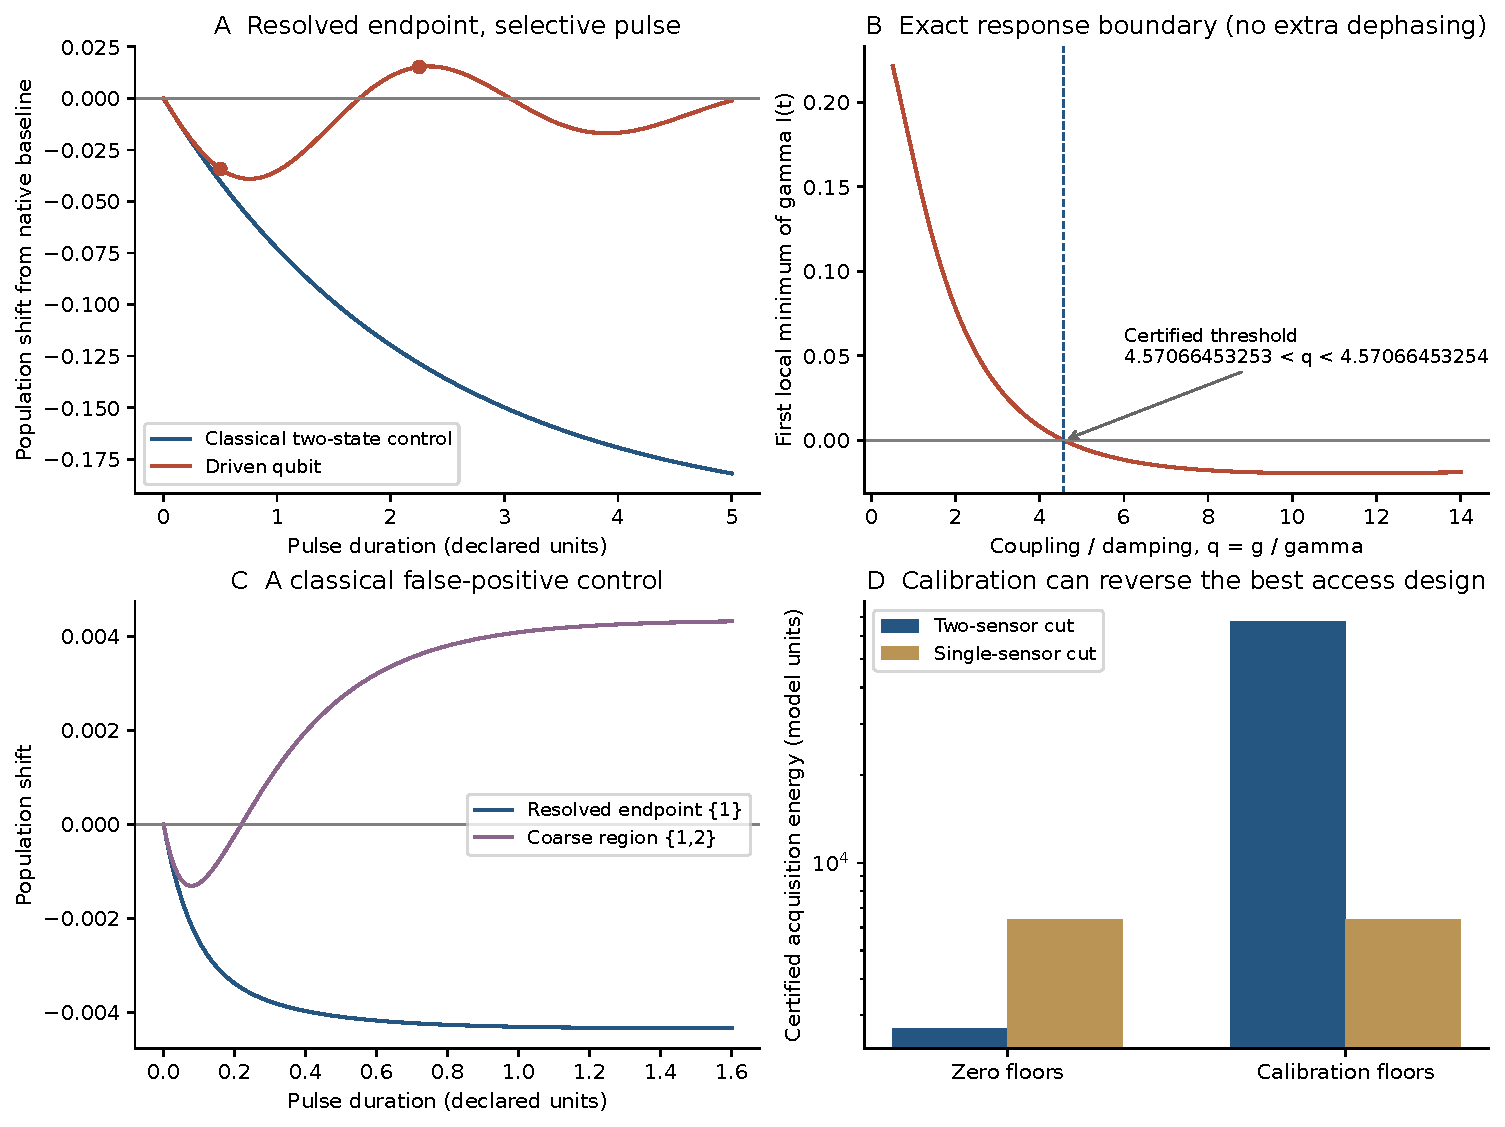
\includegraphics[width=\textwidth]{completion_results.pdf}
\caption{Four consequences of the declared access contracts. A: a driven qubit
crosses its native endpoint baseline, whereas its incoherent control does not.
B: the exact no-extra-dephasing response threshold separates the two regimes.
C: a coarse detector also crosses in a fully classical network; its resolved
endpoint remains protected. D: calibrated floors reverse the preferred current
sensor design at fixed certified accuracy. Curves illustrate proved models;
exact rational certificates, proofs and scope conditions accompany the release.
No panel represents measured experimental data.}
\label{completion:overview}
\end{figure}
